\documentclass[a4paper, 12pt]{article}

% include required packages
\usepackage[a4paper, margin=2cm]{geometry} % Set page margins
\usepackage[round,authoryear]{natbib}      % For citations
\usepackage{url}                           % For formatting URLs
\usepackage{indentfirst}                   % Indent first paragraph of sections
\usepackage{booktabs}                      % For better table formatting
\usepackage{float}                         % For [H] table placement
\usepackage{enumitem}                      % For customising lists
\usepackage{subcaption}                    % For subfigures
\usepackage{graphicx}                      % For includegraphics
\usepackage{tikz}                          % For drawing diagrams
\usetikzlibrary{positioning}               % For relative positioning

% set paragraph and list formatting
\setlength{\parindent}{1.5em}
\setlength{\parskip}{0pt}
\setlist[itemize]{noitemsep,topsep=0pt,parsep=0pt,partopsep=0pt,after=\vspace{0.5em}}


% set title information
\title{A Critical Reflection on the Design of the Web Witchcraft and Wizardry Project}
\author{Edmund Mulligan}
\date{\today}

% document start
\begin{document}

% set bibliography style and page numbering
\bibliographystyle{plainnat}
\pagenumbering{arabic}

\maketitle

\begin{abstract}
\itshape
This essay discusses the design of Web Witchcraft and Wizardry, an educational website teaching children web development. Drawing inspiration from 1960s pop art and magical metaphors, the project employs an Agile development approach with continuous integration and deployment. The essay examines key design elements including colour palettes meeting WCAG 2.2 accessibility standards, typography choices balancing aesthetics with readability, strategic iconography reinforcing the magical theme, purposeful animation enhancing user experience, and comprehensive accessibility features. Digital images created specifically for the project are discussed, along with pedagogical considerations for involving expert educators through working prototypes. Future development will incorporate feedback from students and teachers to create an effective learning platform.
\end{abstract}

\tableofcontents
\newpage

\listoffigures
\newpage

\section{Introduction}
This essay provides a critical reflection on the design of the Web Witchcraft and Wizardry project, which is an educational website aimed at teaching children how to code. The essay discusses the overarching concept behind the project, the design process, and the various elements of the user interface design, including colour, typography, iconography, layout, animation, accessibility, usability and pedagogical considerations. The essay concludes with an indication of how the project will continue to evolve in the future.

\section{Submission Deliverables}
High fidelity user interface designs of the following pages:
\begin{itemize}
    \item Home page
    \item Student Dashboard
    \item Sample Lesson
\end{itemize}
Additional deliverables:
\begin{itemize}
    \item Colour palette and typography specifications for the above pages
    \item Animated GIFs demonstrating the animated elements of the Home page
    \item (For reference) The six digital images submitted in the last assignment
\end{itemize}
These can all be viewed in the Design System section of

\url{https://web.witchcraft-and-wizardry.school/diagnostics}.

A prototype of the website can be accessed at 

\url{https://web.witchcraft-and-wizardry.school}, 

although this is still under construction and may be subject to minor changes while this assignment is being assessed.

\section{Overarching Concept}

\subsection{History and Inspiration}
The Web Witchcraft and Wizardry project, originally used by Kingston University Coder Dojo, was a PDF file with a single HTML file and some inline CSS and JavaScript to get students started. They were then expected to use W3 Schools \citep{w3schools2026} and similar sites to self-study. This was then developed into a web site in GitHub with eight lessons \citep{mulligan2024witchcraftandwizardry}, although minimal consideration was given to appearance or usability (except by accident). The current project aims to redesign the website with a focus on accessibility and visual aesthetics, while maintaining the original Coder Dojo concept of teaching kids to code by coding \citep{coderdojo2026}.

The website draws on the metaphor of computer programming being magical and the programmer being a witch or wizard, which is a common trope both in popular culture (e.g. \cite{rowling1997series}) and in educational contexts (e.g. \cite{kelleher2005lowering, papert1980mindstorms}). Magic as a metaphor for science and education in general is particularly developed in The Science of the Discworld books \citep{pratchett1999science}.

Inspiration for the colours of the new website were taken from the Embodied Mind logo (the author's personal brand), see figure \ref{fig:embodiedmind}. The vibrant style was drawn from 1960's art such as the work of Roy Lichtenstein (e.g. \cite{lichtenstein1963whaam}), Andy Warhol (e.g. \cite{warhol1964marilyn}), and television series such as Batman \citep{batman1966}, Bewitched \citep{bewitched1964} and I Dream of Jeannie \citep{idreamofjeannie1965}. See figures \ref{fig:wham} to \ref{fig:idreamofjeannie} for examples of this style using bold colours and dramatic contrasts. The subdued style, for users who do not want the strident colours of the other two styles, uses a desaturated theme, arguably evoking a pre-colour black and white television look, although this is admittedly a tenuous link, see figure \ref{fig:bbctestcardd}.

The website is designed for children to use, but upon reflection the references for the vibrant style are anchored in the designer's own childhood and may not be as familiar to the current generation of children. However, the style is still vibrant and will hopefully appeal to all users even if they do not understand the references. The design of the website is intended to be inclusive and appealing to a wide range of users, regardless of their familiarity with the specific cultural references. The design also allows users to switch between styles, so they can choose the one that they find most comfortable to use.

\begin{figure}[H]
    \centering
    
\includegraphics[width=0.3\textwidth]{logo-embodied-mind.png}
    \caption{The Embodied Mind logo}
    \label{fig:embodiedmind}
\end{figure}

\begin{figure}[H]
    \centering
    \begin{minipage}[t]{0.48\textwidth}
        \centering
        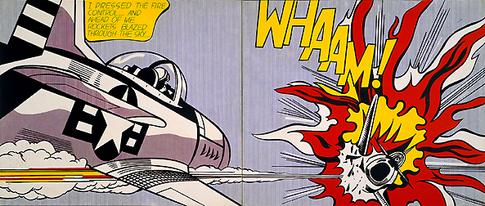
\includegraphics[width=\textwidth]{Roy_Lichtenstein_Whaam.jpg}
        \caption{Roy Lichtenstein's Whaam! \citep{lichtenstein1963whaam}}
        \label{fig:wham}
    \end{minipage}\hfill
    \begin{minipage}[t]{0.48\textwidth}
        \centering
        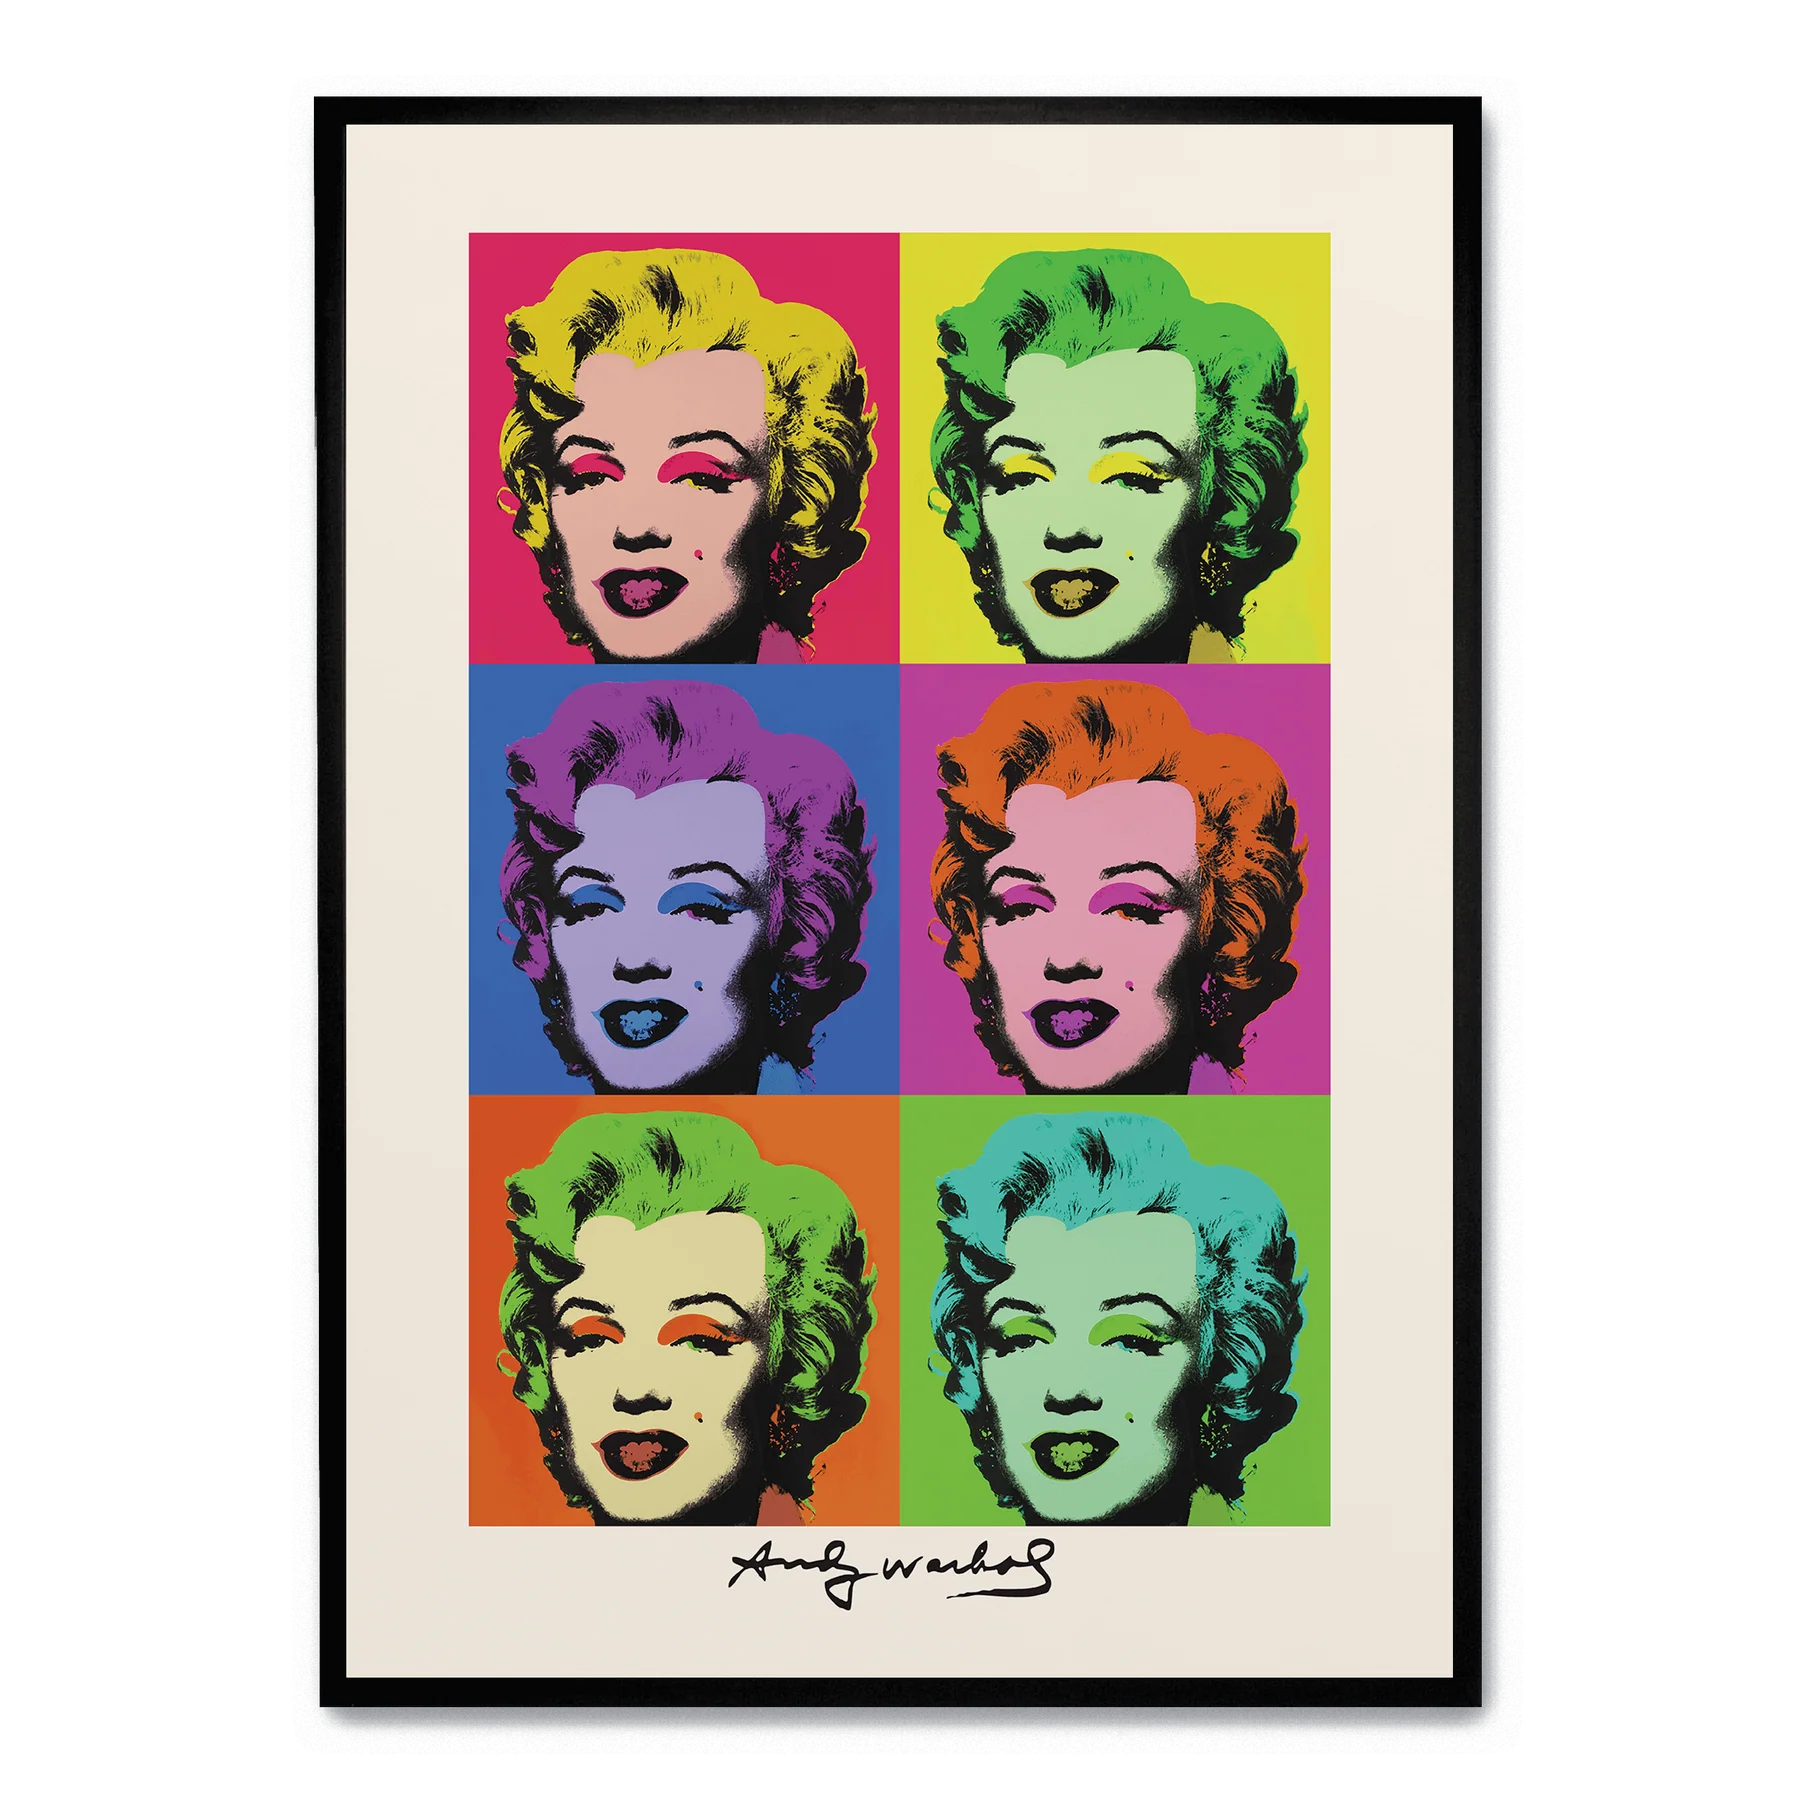
\includegraphics[width=0.85\textwidth]{ShotMarilyn.png}
        \caption{Andy Warhol's Shot Marilyn \citep{warhol1964marilyn}}
        \label{fig:marilyn}
    \end{minipage}
\end{figure}

\begin{figure}[H]
    \centering
    \begin{minipage}[t]{0.45\textwidth}
        \centering
        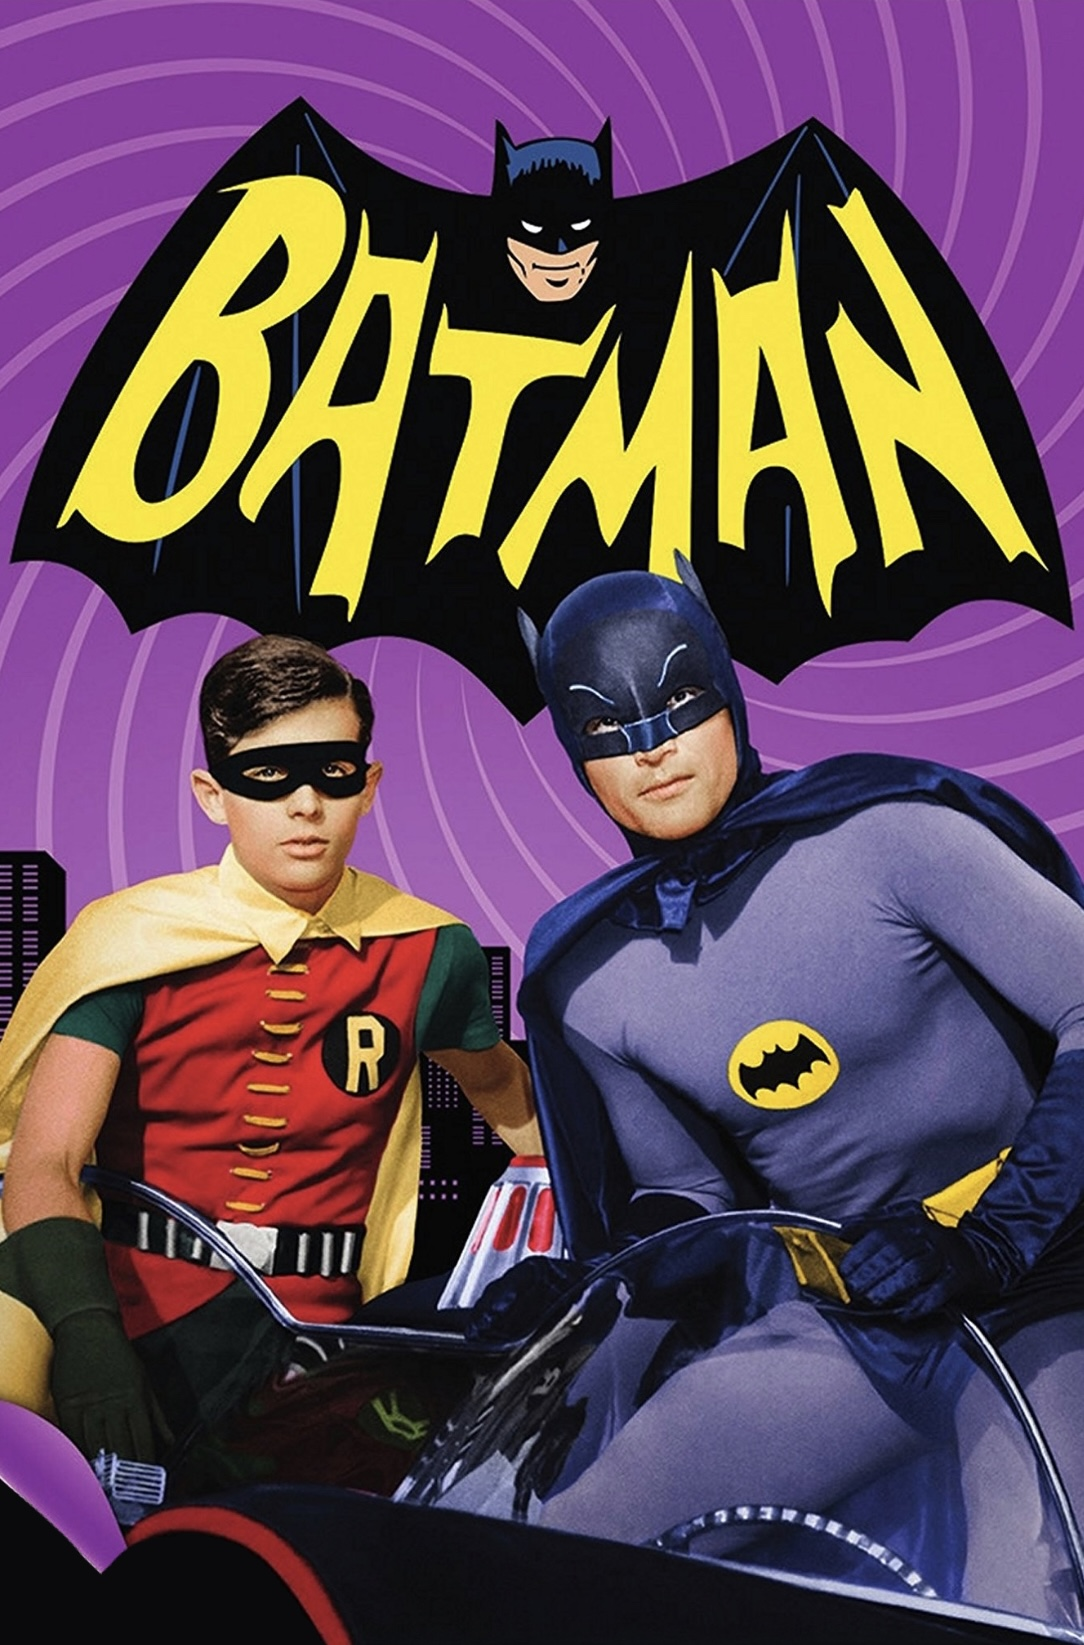
\includegraphics[width=0.5\textwidth]{batman.jpg}
        \caption{Batman \citep{batman1966}}
        \label{fig:batman}
    \end{minipage}\hfill
    \begin{minipage}[t]{0.45\textwidth}
        \centering
        
\includegraphics[width=0.5\textwidth]{bewitched.jpg}
        \caption{Bewitched \citep{bewitched1964}}
        \label{fig:bewitched}
    \end{minipage}
    
    \vspace{1em}
    
    \begin{minipage}[t]{0.45\textwidth}
        \centering
        
\includegraphics[width=0.5\textwidth]{jeannie.jpeg}
        \caption{I Dream of Jeannie \citep{idreamofjeannie1965}}
        \label{fig:idreamofjeannie}
    \end{minipage}\hfill
    \begin{minipage}[t]{0.45\textwidth}
        \centering
        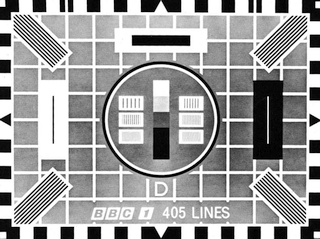
\includegraphics[width=0.75\textwidth]{Testcard_D.png}
        \caption{BBC Test Card D \citep{bbctestcardd}}
        \label{fig:bbctestcardd}
    \end{minipage}
\end{figure}

\subsection{Design Process}
Since the project has a single resource acting as designer, developer and client, an iterative and fluid process was used where design and development were done in parallel. This aligns with the Agile Manifesto \citep{beck2001agile} particularly the second pillar of valuing working software over comprehensive documentation and the seventh principle that working software is the primary measure of progress. Time constraints precluded extensive collaboration with users (another important principle of the Agile Manifesto), but this will be addressed in phase 3 of the project. The development also followed a DevOps approach \citep{allman2018devops} with continuous integration and deployment using GitHub Actions and test automation, which allowed for rapid iteration and testing and refinement of the design. Outstanding work (both development and design) was tracked using GitHub Issues to ensure work was not missed.

The design was also informed by feedback from the first phase of the project and `crit.' from fellow students and tutors. The design and implementation have now reached a stage where the website is functional and visually appealing. It is not yet at the level of a minimum viable product \citep{lenarduzzi2016mvp} as it will require a few more lessons to be written to reach that stage, but it can be considered a working prototype and used to gather feedback from potential users (students and mentors) and experts (teachers). This is an essential part of a robust process to produce usable software \citep{norman2013design} which has been neglected so far. This feedback will be used to further refine the design and implementation of the website, with the aim of creating a final product in the third phase of development, after the Visual Design and Web Project module is completed.

\section{Digital Images}
The digital images can be placed into 4 categories: those created by me for the website, those created by me but not used in the web site, those created by others for the website and those created by others but not specifically for the web site. The first category covers the Embodied Mind logo, the background image of the home page and the sparkling wand used as both the favicon and as an animation at the end of each lesson. It also includes the silhouette icons of a witch and wizard used in page headers which were edited by me from publicly licensed clip art. 

The second category covers images used to demonstrate my competence in image editing and creation and are not directly related to the web site. Images from both categories were discussed in the previous assignment and will not be discussed further here, other than to say they can now be seen in their proper context in the high fidelity designs of the web site.

The third category covers the eight portraits of witches and wizards created for the site \citep{mulligan2025witchesandwizards}. See figure \ref{fig:witchesandwizards} for the images and Appendix \ref{appendix:portraits} for the design brief. They were supplied as JPEG scanned files which were converted to PNG to give them a transparent background.

\begin{figure}[htb]
    \centering
    \begin{subfigure}[b]{0.18\textwidth}
        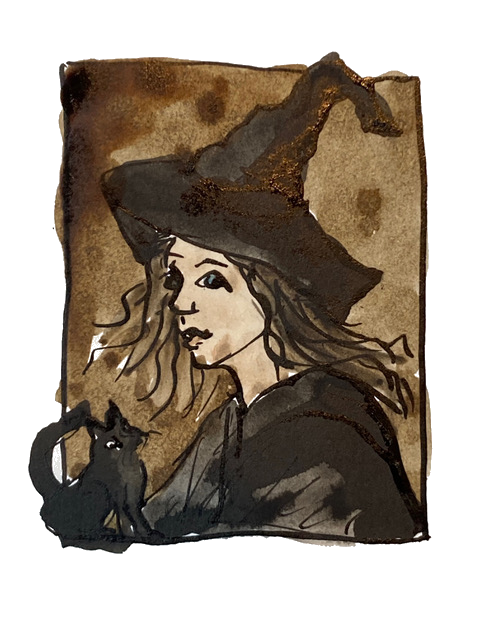
\includegraphics[width=\textwidth]{../images/portraits/rachel-mulligan-witch-young-female.png}
    \end{subfigure}\hfill
    \begin{subfigure}[b]{0.18\textwidth}
        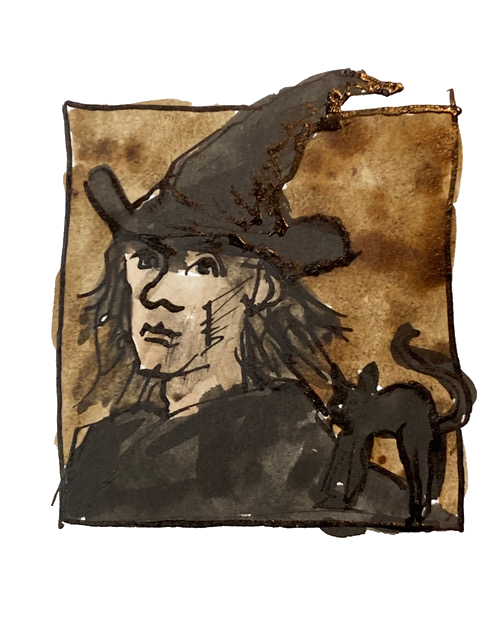
\includegraphics[width=\textwidth]{../images/portraits/rachel-mulligan-witch-young-male.png}
    \end{subfigure}\hfill
    \begin{subfigure}[b]{0.18\textwidth}
        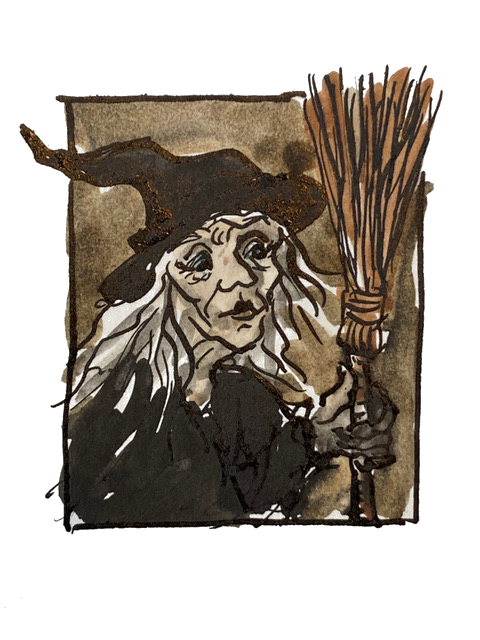
\includegraphics[width=\textwidth]{../images/portraits/rachel-mulligan-witch-old-female.png}
    \end{subfigure}\hfill
    \begin{subfigure}[b]{0.18\textwidth}
        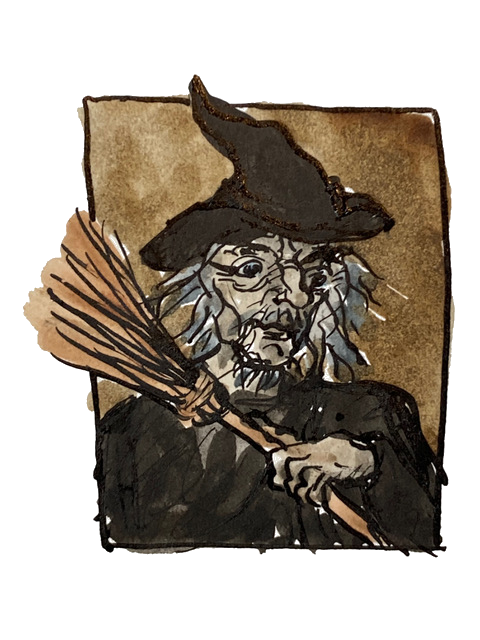
\includegraphics[width=\textwidth]{../images/portraits/rachel-mulligan-witch-old-male.png}
    \end{subfigure}
    
    \begin{subfigure}[b]{0.18\textwidth}
        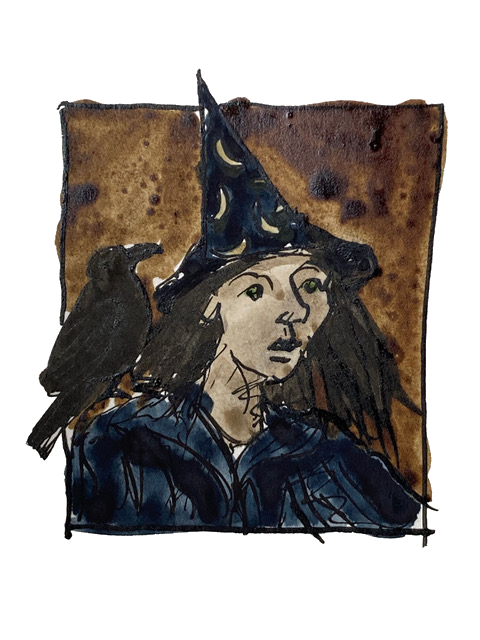
\includegraphics[width=\textwidth]{../images/portraits/rachel-mulligan-wizard-young-female.png}
    \end{subfigure}\hfill
    \begin{subfigure}[b]{0.18\textwidth}
        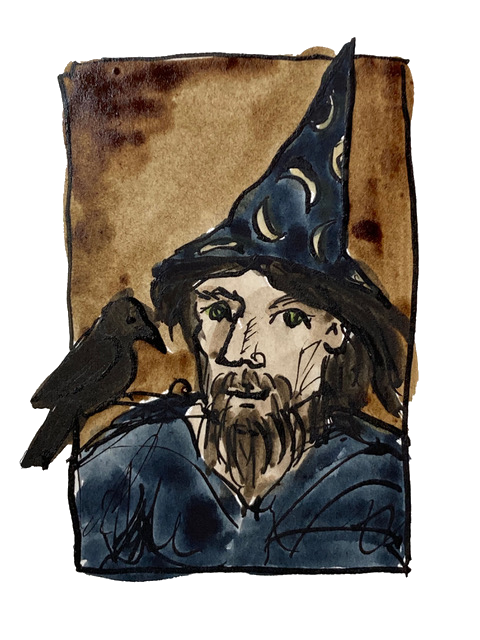
\includegraphics[width=\textwidth]{../images/portraits/rachel-mulligan-wizard-young-male.png}
    \end{subfigure}\hfill
    \begin{subfigure}[b]{0.18\textwidth}
        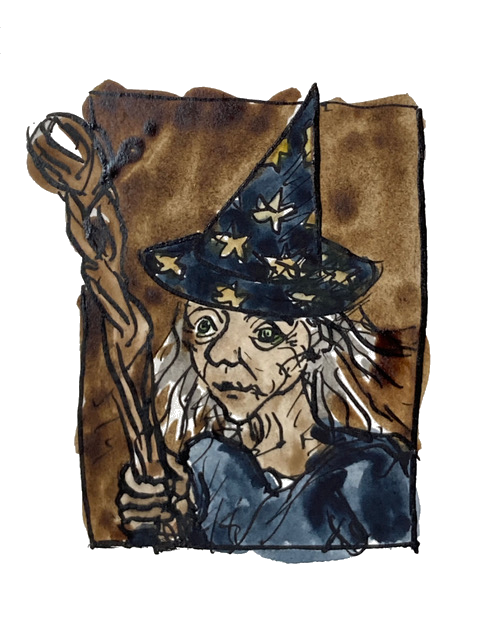
\includegraphics[width=\textwidth]{../images/portraits/rachel-mulligan-wizard-old-female.png}
    \end{subfigure}\hfill
    \begin{subfigure}[b]{0.18\textwidth}
        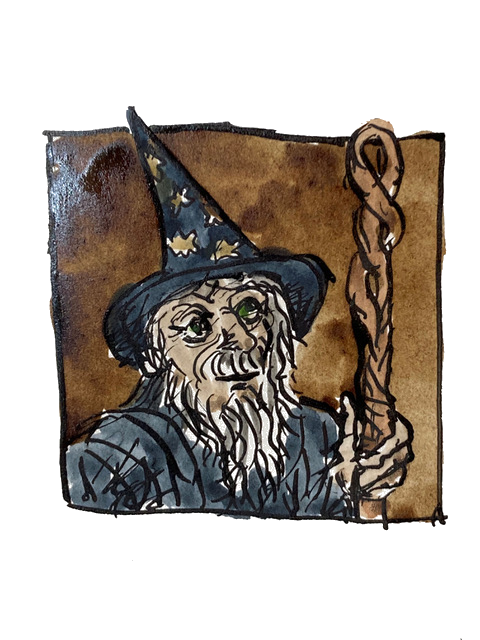
\includegraphics[width=\textwidth]{../images/portraits/rachel-mulligan-wizard-old-male.png}
    \end{subfigure}
    \caption{Eight portraits of witches and wizards by Rachel Mulligan \citep{mulligan2025witchesandwizards}}
    \label{fig:witchesandwizards}
\end{figure}

The final category covers icons from Font Awesome used under a Font Awesome Pro license and which are discussed under Iconography below.

\section{User Interface Designs}

The high fidelity user interface designs are presented on an interactive page since each page design requires at least 48 images to cover the combination of styles, themes and sample viewport sizes. It can also be viewed as a working prototype at \url{https://web.witchcraft-and-wizardry.school} which will give a more dynamic experience of the design. Individual elements of the design are discussed below.

\subsection{Colour}
Generally, the first thing that people notice about a design is the colour scheme \citep{lindgaard2006attention}, so arguably this is the most important aspect of the design, although see, for example, \cite{tschichold1991new} for a dissenting view. Having selected colour schemes based on the criteria outlined in the History and Inspiration section, the next challenge is to choose specific colours that meet the WCAG 2.2 guidelines for contrast and accessibility \citep{caldwell2024}. With so many colours in the different themes and styles, this was a non-trivial task and required the development of a custom tool to quickly check the contrast of possible combinations of colours. See \url{https://web.witchcraft-and-wizardry.school/diagnostics/colourPalette.html}. It uses colour variables from the CSS of the website so the impact of any colour changes can be immediately assessed. The final selection is documented at \url{https://web.witchcraft-and-wizardry.school/diagnostics/colourSwatches.html}. and all contrasts meet at least AA standards, with most meeting AAA.

The phase 1 website submitted last term used named CSS colours, but that was too inflexible for the current design. RGB hex codes were tried but again that was too restrictive and eventually relative colours and a HSL colour scheme were used to allow for easier maintenance. This has the limitation of being a new CSS feature but has been supported by all major browsers since 2024 \citep{caniuse2026}. Kevin Powell's YouTube tutorials \citep{powell_youtube} recommends using fallback colours for unsupported browsers, and this will be incorporated in the next phase of development to make the site more robust.

\subsection{Typography}

Compared to colour, typography is relatively straightforward for this website, The first requirement was for a legible font for the body text and after that a suitable `magic-y' font for the headings. A search of Google Fonts \citep{googlefonts2026} led to the selection of Open Sans and Cinzel/Cinzel Decorative for these purposes, respectively. `Magic-y' is, admittedly, a subjective term and for the purposes of this project, it refers to a font that evokes a sense of fantasy or enchantment, while still being highly legible (ruling out overly decorative or script fonts). A monospace font was also needed for code snippets and this was fulfilled by Fira Code. All fonts are freely usable under the Open SIL license \citep{silofl2007}.

The size of fonts was effectively delegated to the browser using the CSS clamp() function to allow for responsive scaling. This facilitates a responsive design that can meet WCAG 2.2 guidelines for text size and readability \citep{caldwell2024} without needing to specify multiple font sizes for different viewport sizes.

The only remaining issue, which was pointed out in the `crit' session is that Cinzel is a capital only font. This looks fine for headlines but does present accessibility issues for people with dyslexia and other reading difficulties \citep{rello2013dyslexia}. For this reason, additional fonts of Marcellus and Cormorant Garamond were selected to use in menu items and button labels respectively instead of Cinzel. This is a good example of incorporating user feedback to achieve accessibility, with pragmatism trumping pure design, in line with good web design practice \citep{norman2013design}.

Typographical choices are documented at 

\url{https://web.witchcraft-and-wizardry.school/diagnostics/typography.html}.

\subsection{Layout}
The main design challenge with respect to layout is how to handle the large amount of text in the lessons. The solution adopted is to break the lessons into sections and use a navigation panel to allow users to see one section at a time without excessive scrolling (see the sample lesson high fidelity prototype). Where large blocks of text are unavoidable, such as in the Frequently Asked Questions page, sections are by default hidden and are toggled on and off with navigation buttons. This allows users to focus on the information they need without being overwhelmed by too much information at once.

The ideal width for text is generally considered to be around 50-75 characters per line \citep{bringhurst2013elements}, and responsive design, using the CSS clamp() function and ch units, has been used, along with grid layouts, to adjust the number of columns of text on the screen dynamically to maintain optimum readability without needing to specify different layouts in media queries.

One problem with early versions of the web site was that very narrow viewports rendered poorly due to fragile CSS. For this reason a CSS based warning was added at viewports of less than 200px width to encourage users to use a larger screen for the best experience. The CSS is now much more robust and the pages render correctly at narrow widths, but the warning remains as a helpful nudge to users to use a larger screen. An assumption has been made that, since this is a web site teaching web development, most users will be using a computer with a reasonably large screen, so a `mobile-first' design approach was not taken. However, the design is responsive and will work on mobile devices, albeit with a warning about the suboptimal experience at very narrow widths.

\subsection{Iconography}
Although this project is called Web Witchcraft and Wizardry, apart from the Gallery of portraits and the Facts about Witches and Wizards page, there is not much witchy or wizardly on the site. To some extent this will be addressed when the lessons are written as these will make the metaphor of programming as casting spells very explicit. However the magical theme can be greatly enhanced through the use of appropriate iconography \citep{horton1994icon}. This is most obviously done with the witch and wizard in the header of each page, but also with the use of the wand icon. This is used both for navigation and in the Frequently Asked Questions page to indicate whether an answer section is expanded or collapsed (see Figure \ref{fig:wands}). The wand icons are from Font Awesome Pro \citep{fontawesome2026} and are used under the Font Awesome Pro license.

\begin{figure}
    \centering
    \begin{subfigure}[b]{\textwidth}
        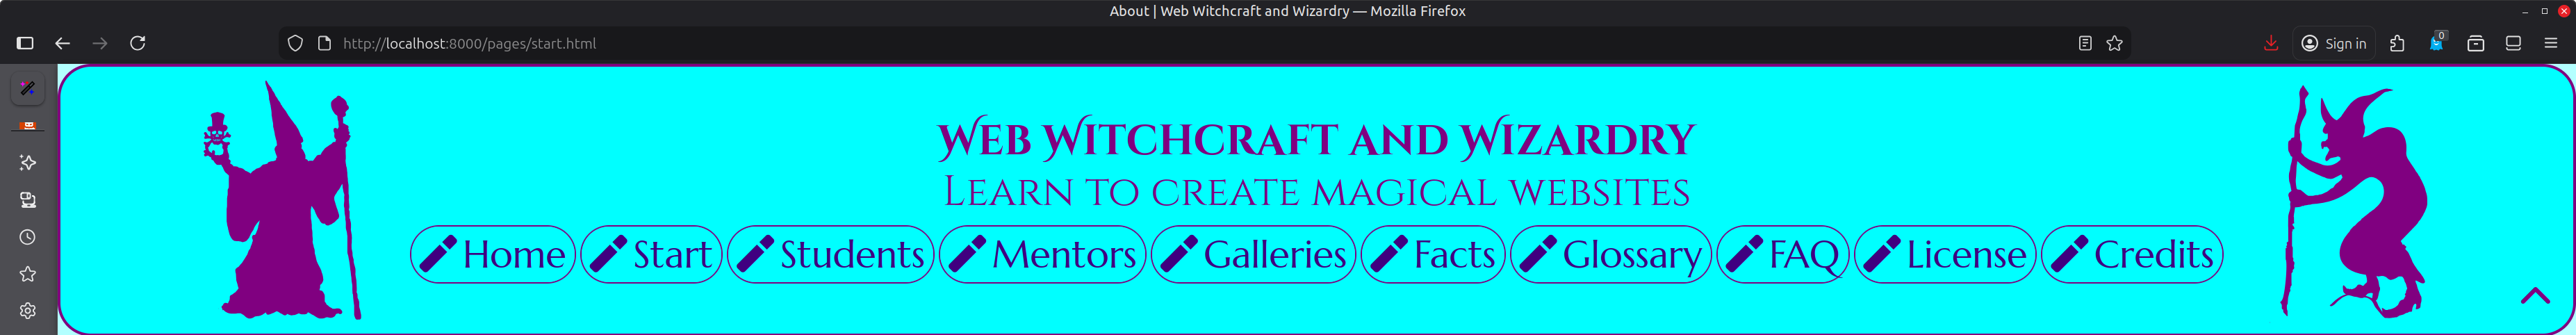
\includegraphics[width=\textwidth]{nav-menu-1.png}
        \caption{Wand used in navigation}
        \label{fig:wand-navigation}
    \end{subfigure}\hfill
    \begin{subfigure}[b]{\textwidth}
        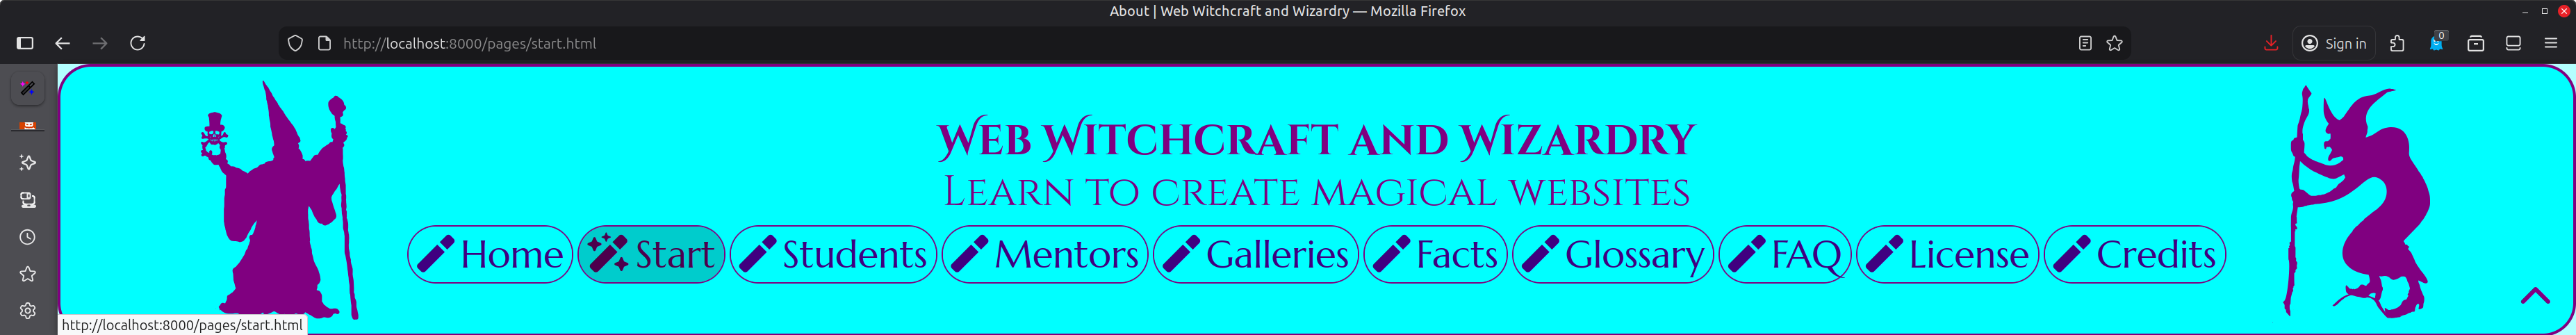
\includegraphics[width=\textwidth]{nav-menu-2.png}
        \caption{Wand used in navigation when hovered}
        \label{fig:wand-navigation-hover}
    \end{subfigure}
    \begin{subfigure}[b]{\textwidth}
        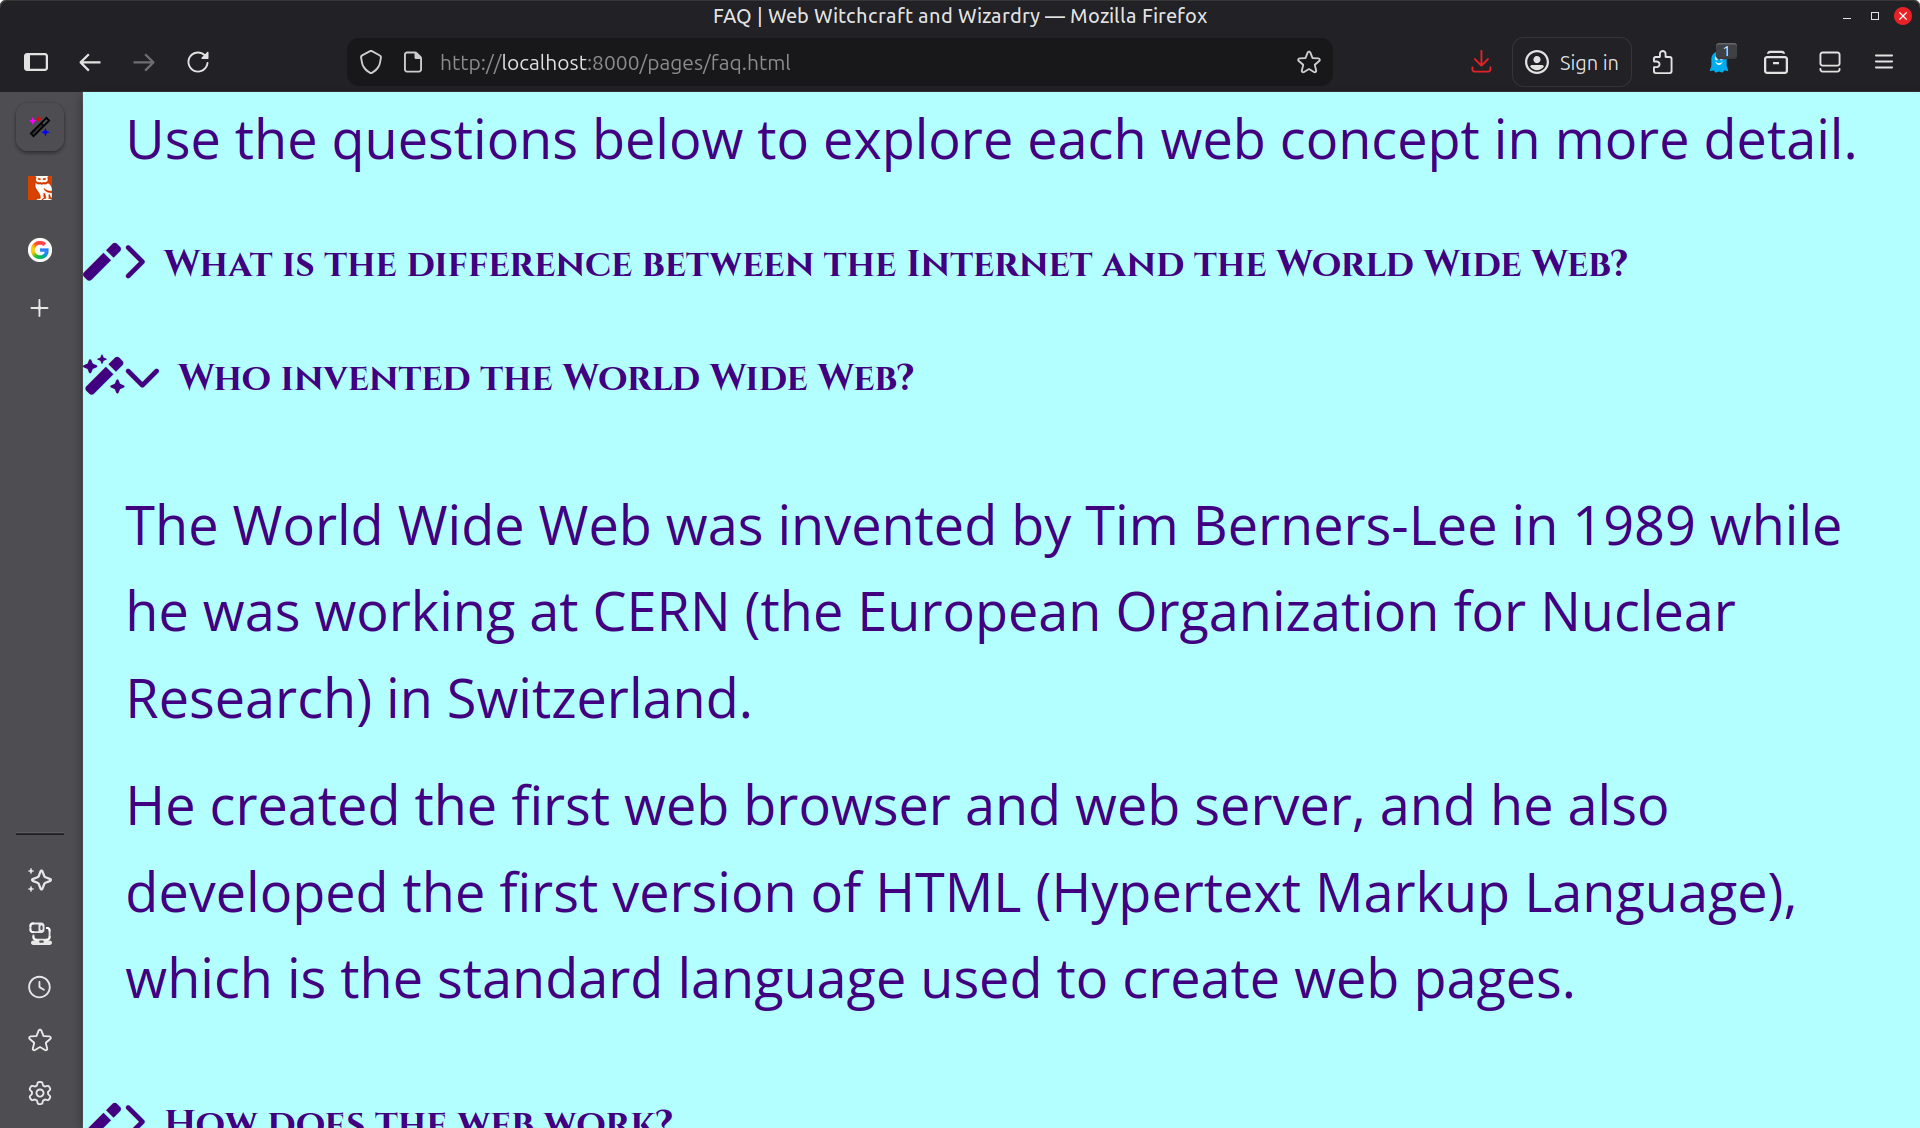
\includegraphics[width=\textwidth]{wand_iconography.png}
        \caption{Wand used in FAQ page to indicate expanded/collapsed sections}
        \label{fig:wand-faq}
    \end{subfigure}
    \caption{Wand icons used in Web Witchcraft and Wizardry \citep{fontawesome2026}}
    \label{fig:wands}
\end{figure}

Font Awesome also provides many other magic-adjacent icons (see

\url{https://web.witchcraft-and-wizardry.school/pages/gallery.html} 

for examples) which will be used in lessons as soon as images are introduced to the students. The magical imagery will really start to fly, so to speak, after CSS animation and JavaScript have been covered and students can start creating interactive and animated web pages.

\subsection{Animation}
There is very little animation used on this site and that is deliberate. The principle of `less is more' applies to animation as much as it does to other design elements \citep{norman2013design}, and a conscious choice has been made to only use animation when it is in service to the user experience. Thus the animations used are mostly very subtle, such as buttons increasing in size slightly when hovered over, navigation wands sparkling when hovered and scrolling through images in the gallery page. 

There are two exceptions to this principle. The first is using an animated sparkling wand at the end of each lesson as a `reward' for completing the lesson. The second exception is on the home page where two very obvious animations are used. One is when transitioning between themes and styles and the other is in the display of random portraits which fade in and out. The reason for this is that the home page is the `shop window' of the website and needs to be visually engaging to encourage users to explore the site further. The animations are designed to be fun and engaging without being overwhelming or distracting. Nevertheless, there is a button to disable the animations for users who prefer a more static experience. The page also respects the prefers-reduced-motion media query to disable animations for users who have set that preference in their operating system settings. The animations on the home page have been recorded as animated GIF files in the high fidelity designs, both because that was a requirement of this assignment, but also to allow documentation of the animations in a static format.

Animation will be covered in the Web Project Code and Report submission, but the principle I have followed is one of separation of concerns: animation is part of the visual appearance of the web site so should be (and has been) implemented in CSS without using JavaScript where possible. Since some CSS animation features are not yet supported by all browsers, JavaScript fallback animations are still necessary in some cases, such as the image scrollers in the gallery page.

\subsection{Accessibility}
Accessibility has been mentioned already in several sections, and it is a primary goal of this website redesign to provide an accessible experience to all users of the site. This not only makes the site useable by people who have disabilities or other restrictions, but also makes the experience better for all users who want to use their computer or device in the way they want to \citep{story1998universal}. 

\subsection{Usability}
Designing good usability generally requires input from actual users \citep{norman2013design}. With the resource and time constraints of the project, this has not been possible so far, but will be a major focus of the next phase of development. One potential usability problem has been identified and that is a `Desire Line' \citep{lynch1960image} where students can access the lessons without having selected an avatar on the Student Dashboard. This is not a critical flaw as the lessons are still accessible and usable without an avatar, but future lessons will make more use of the avatar so at that point it will be necessary to devise a mechanism to encourage students to select an avatar before accessing the lessons. Their avatar choice is saved in local storage so it only needs to be selected once, but it is still important to encourage students to make that selection to get the full experience of the site.

\subsection{Pedagogical Considerations}
Web Witchcraft and Wizardry is an educational website and as such it should have significant input to its design and content from expert educators (i.e. teachers). Since most teachers are not primarily web developers, the best way to allow them to contribute their expertise is to give them a working application to comment on \citep{schuler1993participatory}. Thus the next phase of development will explicitly include collaboration with teachers who have expressed an interest in the project.

There are two main types of users of the web site. The first is the students who want to learn how to create web pages. These may either be working on their own remotely or taking part in a Coder Dojo or other computer programming club. These latter students are supported by mentors, who are generally volunteers and may not have specific expertise in web development. So the mentors are the second class of users and for each lesson there will be the main student page and a secondary page for the mentors with learning outcomes for that lesson and, as best as can be anticipated, common pitfalls that students may encounter. The content of these mentor pages will be developed in phase three, after the lessons have been piloted with real students at Kingston University Coder Dojo and the issues they encounter have been observed.

\section{Conclusion}
This essay has provided a critical reflection on the design of the Web Witchcraft and Wizardry project, which is an educational website aimed at teaching children how to create web sites. While the design is complete as far as it goes, sufficient at least to build a working prototype, there is still work required to solicit and incorporate feedback from students and educators and to write the lessons and mentor guides. The next phase of development will focus on these aspects of the project, with the aim of creating a final product that is exciting to use and rigorously effective at teaching good coding practice to the next generation of web developers.

% Include word count N.B. Run wordcount.sh to generate wordcount.txt before compiling
\section*{Word count}
Word count: \input{essay-2-wordcount.txt} words (excluding references)
\\
\bibliography{EdmundLibrary}

% include appendices
\newpage
\appendix
\section*{Appendices}
\section{Design Brief for Witches and Wizards Artwork}\label{appendix:portraits}

Please create a series of portraits of witches and wizards for the Web Witchcraft and Wizardry project. The portraits should be in a cartoon-like but detailed art style, suitable for use on a website. The characters should be a combination of witch and wizard, young and old, and female and male (eight in total). The portraits should be designed according to the following rules:

\subsection*{Witches}

\begin{itemize}
    \item Wear pointed hats (various styles but always black) and black clothes
    \item May accessorise with a wand, crystal ball or broomstick
    \item May have a black cat familiar
\end{itemize}

\subsection*{Wizards}

\begin{itemize}
    \item Wear wide-brimmed hats or elaborate headgear and long robes
    \item May accessorise with a staff, spell book or skull
    \item May have a raven familiar
    \item Are generally more formal in appearance than witches
\end{itemize}

\subsection*{In addition}

\begin{itemize}
    \item Witches have wild or flowing hair when visible
    \item Male Wizards have beards (various styles appropriate to age and character)
    \item Male Witches are clean shaven
\end{itemize}

These portraits will be used by kids as avatars so nothing too scary, sinister or suggestive.

Thank you and please don't spend too much time on this.

\end{document}
